\section{Experiments}

\subsection{Experimental Setup}

\textbf{Datasets.}
We evaluate continuous-sensor forecasting on HumanActivity, MHEALTH,
OPPORTUNITY, PAMAP2, USC-HAD, and REALDISP
\citep{rubanova2019latent,uci_mhealth,uci_opportunity,uci_pamap2,usc_had,uci_realdisp}. They span
6--117 variables, compact physiological traces, long activity streams, and
heterogeneous body placements (Table~\ref{tab:v665-data-main}). Released
subjects define disjoint training, validation, and test partitions; all
sessions of one subject remain in one partition. The main benchmark retains
released timestamps and finite-value availability and does not inject an
artificial observation mask. Activity labels and subject identifiers are never
model inputs. Mean squared error (MSE) is the primary endpoint and mean
absolute error (MAE) is the complementary endpoint, both evaluated on
available future targets. The task
is continuous sensor forecasting rather than activity recognition or clinical
decision support.

\begin{table}[t]
\centering
\setlength{\tabcolsep}{4pt}
\caption{Datasets and forecasting dimensions. $D/L/H/P$ denote variables,
history, horizon, and patch length.}
\label{tab:v665-data-main}
\begin{tabular}{@{}lrrrrr@{}}
\toprule
Dataset & $D$ & Train/Val/Test & $L$ & $H$ & $P$ \\
\midrule
HA   & 12  & 3/1/1 & 3000 & 300 & 60 \\
MH   & 23  & 7/1/2 & 250  & 50  & 10 \\
OPP  & 64  & 2/1/1 & 300  & 60  & 12 \\
PAM  & 37  & 6/1/2 & 500  & 100 & 20 \\
USC  & 6   & 9/2/3 & 300  & 60  & 15 \\
REAL & 117 & 1/1/1 & 500  & 100 & 25 \\
\bottomrule
\end{tabular}
\end{table}


For compact table headings, we abbreviate HumanActivity as HA, MHEALTH as MH,
OPPORTUNITY as OPP, PAMAP2 as PAM, USC-HAD as USC, and REALDISP as REAL.

\textbf{Baselines and protocol.}
The complete benchmark includes APN, KAFNet, GraFITi, tPatchGNN, and PatchTST
\citep{apn2026,kafnet2026,grafiti2024,tpatchgnn2024,nie2023patchtst}. For every
method--dataset pair, six validation trials vary learning rate, hidden width,
and dropout under the same optimizer and objective. Validation MSE, with
MAE as tie-breaker, freezes one configuration before test evaluation. The
search varies common optimization and capacity axes rather than
architecture-specific components. The
complete matrix is reported below. Independently, validation MSE with a
validation-MAE tie-break freezes one public comparator per dataset. The same
comparator is used for both test metrics and all five matched runs; test errors
never determine its identity. No model or hyperparameter is reselected per
run. Paired bootstrap intervals over the five optimization runs quantify
run-to-run stability, not uncertainty over new subjects. Final-model component controls use three
repeated runs on the four core datasets.

\textbf{Implementation.}
All models use Adam, at most 20 epochs, and the common forecasting objective
$\mathrm{MSE}+0.5\mathrm{MAE}$. The six-trial search and run-5401 public
confirmation use patience five; final MESANet and added run-5402--5405
confirmations use patience six. MESANet uses four causal supports initialized
at $\{0.5,1,2,4\}$ times the base patch width, DCT rank $R=\min(4,H)$, and
fixed overlap $\rho=0.5$. Its validation-frozen width/dropout pairs for
HA/MH/OPP/PAM/USC/REAL are $48/0$, $72/.05$, $64/.1$, $96/.05$, $32/.05$,
and $144/.05$, respectively.
Dataset dimensions, exact search spaces, and executable commands are in the
supplement.

\subsection{Main Results}

\begin{table*}[t]
\centering
\setlength{\tabcolsep}{2.35pt}
\caption{Run-5401 validation-frozen wearable IMTS benchmark. Public rows use
the shared six-trial search; MESANet uses its final frozen configuration.
Lower is better; best results are bold and second-best results are underlined.}
\label{tab:v665-main}
\begin{tabular}{@{}l*{12}{r}@{}}
\toprule
\multirow{2}{*}{Method} & \multicolumn{2}{c}{HA} & \multicolumn{2}{c}{MH}
& \multicolumn{2}{c}{OPP} & \multicolumn{2}{c}{PAM}
& \multicolumn{2}{c}{USC} & \multicolumn{2}{c}{REAL} \\
& MSE & MAE & MSE & MAE & MSE & MAE & MSE & MAE & MSE & MAE & MSE & MAE \\
\midrule
APN       & 0.0549 & 0.1381 & 0.7049 & 0.4789 & 0.8362 & 0.6387 & 0.8886 & 0.5037 & 0.7204 & 0.4384 & 0.8480 & 0.5594 \\
KAFNet    & \textbf{0.0450} & \underline{0.1156} & 0.7019 & 0.4734 & 0.7921 & 0.6057 & 0.8696 & 0.5000 & 0.7193 & 0.4360 & 0.7774 & 0.5441 \\
GraFITi   & 0.0459 & 0.1193 & 0.6786 & 0.4651 & 0.7404 & 0.5881 & \underline{0.8445} & \underline{0.4573} & 0.7189 & 0.4336 & \underline{0.6128} & \underline{0.4482} \\
tPatchGNN & 0.0462 & 0.1199 & 0.6630 & 0.4479 & \underline{0.7138} & 0.5652 & 0.8605 & 0.4697 & 0.7254 & 0.4444 & 0.7410 & 0.4860 \\
PatchTST  & 0.0836 & 0.1889 & \underline{0.5323} & \underline{0.4012} & 0.7174 & \underline{0.5575} & 0.8501 & 0.4630 & \textbf{0.6168} & \textbf{0.3903} & \textbf{0.6029} & 0.4540 \\
\textbf{MESANet} & \underline{0.0454} & \textbf{0.1138} & \textbf{0.5282} & \textbf{0.3908} & \textbf{0.6865} & \textbf{0.5517} & \textbf{0.8416} & \textbf{0.4567} & \underline{0.6493} & \underline{0.4051} & 0.6139 & \textbf{0.4314} \\
\bottomrule
\end{tabular}
\end{table*}


Table~\ref{tab:v665-main} gives full method coverage after freezing each
method's validation-selected configuration. It is the complete descriptive
test matrix; it does not select the comparator used for repeated comparison.

\begin{table*}[t]
\centering
\setlength{\tabcolsep}{2.2pt}
\caption{Validation-frozen five-run comparison. One public comparator is
selected per dataset by validation MSE and used for both test metrics. Values
are mean $\pm$ standard deviation; positive gains favor MESANet. $\dagger$
marks a paired bootstrap interval over the five optimization runs above zero.}
\label{tab:v671-validation-frozen}
\begin{tabular}{@{}llrrrrrr@{}}
\toprule
Dataset & Frozen public comparator & Public MSE & MESANet MSE & Gain & Public MAE & MESANet MAE & Gain \\
\midrule
HA & KAFNet & 0.0449$\pm$0.0001 & 0.0453$\pm$0.0003 & -0.85\% & 0.1148$\pm$0.0005 & 0.1134$\pm$0.0004 & +1.19\%$^\dagger$ \\
MH & PatchTST & 0.5369$\pm$0.0069 & 0.5267$\pm$0.0039 & +1.89\%$^\dagger$ & 0.4040$\pm$0.0047 & 0.3901$\pm$0.0016 & +3.43\%$^\dagger$ \\
OPP & tPatchGNN & 0.7098$\pm$0.0061 & 0.6944$\pm$0.0048 & +2.17\%$^\dagger$ & 0.5606$\pm$0.0046 & 0.5475$\pm$0.0024 & +2.33\%$^\dagger$ \\
PAM & GraFITi & 0.8455$\pm$0.0024 & 0.8432$\pm$0.0034 & +0.27\% & 0.4595$\pm$0.0023 & 0.4580$\pm$0.0024 & +0.34\% \\
USC & PatchTST & 0.6227$\pm$0.0078 & 0.6520$\pm$0.0038 & -4.70\% & 0.3923$\pm$0.0025 & 0.4051$\pm$0.0008 & -3.24\% \\
REAL & PatchTST & 0.6221$\pm$0.0108 & 0.6141$\pm$0.0024 & +1.28\% & 0.4447$\pm$0.0053 & 0.4321$\pm$0.0026 & +2.84\%$^\dagger$ \\
\bottomrule
\end{tabular}
\end{table*}


Table~\ref{tab:v671-validation-frozen} gives the validation-frozen repeated
comparison. MESANet improves mean error in 9 of 12 metric cells and both
metrics on four datasets. Six cells have paired bootstrap intervals over the
five optimization runs above zero. The largest dual-metric gains occur on
MHEALTH ($1.89\%$ MSE,
$3.43\%$ MAE), OPPORTUNITY ($2.17\%$, $2.33\%$), and REALDISP ($1.28\%$,
$2.84\%$); PAMAP2 adds smaller gains ($0.27\%$, $0.34\%$). Dagger-marked
intervals are run-level stability checks for the frozen contrasts rather than
population-level uncertainty statements.

The two boundary datasets sharpen the scope. HumanActivity improves MAE by
$1.19\%$ but trails KAFNet MSE by $0.85\%$, indicating that waveform-aware
forecasting reduces typical error without improving the largest deviations.
On USC-HAD, PatchTST remains better by $4.70\%$ MSE and $3.24\%$ MAE. Thus,
the gains are dataset dependent: the experiments do not establish a universal
advantage over compact regular-patch representations or identify one dataset
property that predicts the gain.

\subsection{Ablation Studies}
\label{sec:ablation}

\begin{table*}[t]
\centering
\setlength{\tabcolsep}{1.05pt}
\caption{Three-run component controls on four core datasets for fixed-$\rho$
MESANet. Cells are run means; average degradation is the geometric mean of 12
paired control/MESANet run ratios. Positive values favor the complete model.}
\label{tab:v671-controls}
\begin{tabular}{@{}l*{4}{rr}rrrr@{}}
\toprule
& \multicolumn{2}{c}{HA} & \multicolumn{2}{c}{MH} & \multicolumn{2}{c}{OPP} & \multicolumn{2}{c}{PAM} & \multicolumn{2}{c}{Avg. deg.} & \multicolumn{2}{c}{Full wins} \\
Variant & MSE & MAE & MSE & MAE & MSE & MAE & MSE & MAE & $\Delta$MSE & $\Delta$MAE & MSE & MAE \\
\midrule
MESANet ($\rho=0.5$) & 0.0455 & 0.1136 & 0.5258 & 0.3896 & 0.6931 & 0.5481 & 0.8442 & 0.4586 & -- & -- & -- & -- \\
single coordinate (matched) & 0.0453 & 0.1152 & 0.6163 & 0.4210 & 0.7023 & 0.5484 & 0.8506 & 0.4614 & +4.51\% & +2.47\% & 3/4 & 4/4 \\
w/o waveform coordinate & 0.0453 & 0.1140 & 0.6207 & 0.4241 & 0.6965 & 0.5461 & 0.8430 & 0.4576 & +4.23\% & +2.06\% & 2/4 & 2/4 \\
w/o multiresolution & 0.0460 & 0.1145 & 0.5443 & 0.4009 & 0.6975 & 0.5484 & 0.8476 & 0.4605 & +1.43\% & +1.01\% & 4/4 & 4/4 \\
w/o affine anchor & 0.0455 & 0.1193 & 0.5515 & 0.4069 & 0.6813 & 0.5415 & 0.8475 & 0.4669 & +0.90\% & +2.46\% & 3/4 & 3/4 \\
shared transfer (matched) & 0.0459 & 0.1145 & 0.5237 & 0.3888 & 0.6980 & 0.5468 & 0.8467 & 0.4589 & +0.37\% & +0.09\% & 3/4 & 2/4 \\
random basis (matched) & 0.0473 & 0.1210 & 0.5399 & 0.3998 & 0.6999 & 0.5499 & 0.8636 & 0.4648 & +2.50\% & +2.67\% & 4/4 & 4/4 \\
\bottomrule
\end{tabular}
\end{table*}


Table~\ref{tab:v671-controls} evaluates the fixed-$\rho$ implementation rather than
an earlier prototype. A parameter-matched single-coordinate model increases
the geometric mean of paired run--dataset MSE/MAE ratios by
$4.51\%/2.47\%$, consistent with a dual-coordinate benefit beyond parameter
count alone. Removing the ordered waveform coordinate causes $4.23\%/2.06\%$
average degradation. The complete model wins MSE on two datasets and MAE on
two, but MHEALTH is the only dual-metric win; the waveform contribution is
therefore regime dependent rather than uniformly beneficial. Removing the
multiresolution coordinate increases MSE on all four datasets and produces
$1.43\%/1.01\%$ geometric-mean degradation. Removing affine anchoring costs
$0.90\%/2.46\%$ under the same aggregation and degrades both metrics on three datasets;
OPPORTUNITY is the boundary case. Thus, canonicalization and restoration are
predictive components of the evaluated backbone.

The deployed model fixes $\rho=0.5$; learned- and endpoint-overlap variants are
reported only as sensitivity controls in the supplement. A parameter-matched
random orthonormal basis degrades MSE/MAE by $2.50\%/2.67\%$ and loses on all
four datasets. This supports the ordered DCT coordinate relative to the
matched random-basis control, rather than attributing the result to arbitrary
two-head capacity. Sharing variable transfer is nearly tied
($0.37\%/0.09\%$ aggregate degradation with mixed per-dataset wins); these
three-run controls provide no evidence that separate transfer parameters
improve accuracy.

\subsection{Parameter Sensitivity}

\begin{figure}[t]
\centering
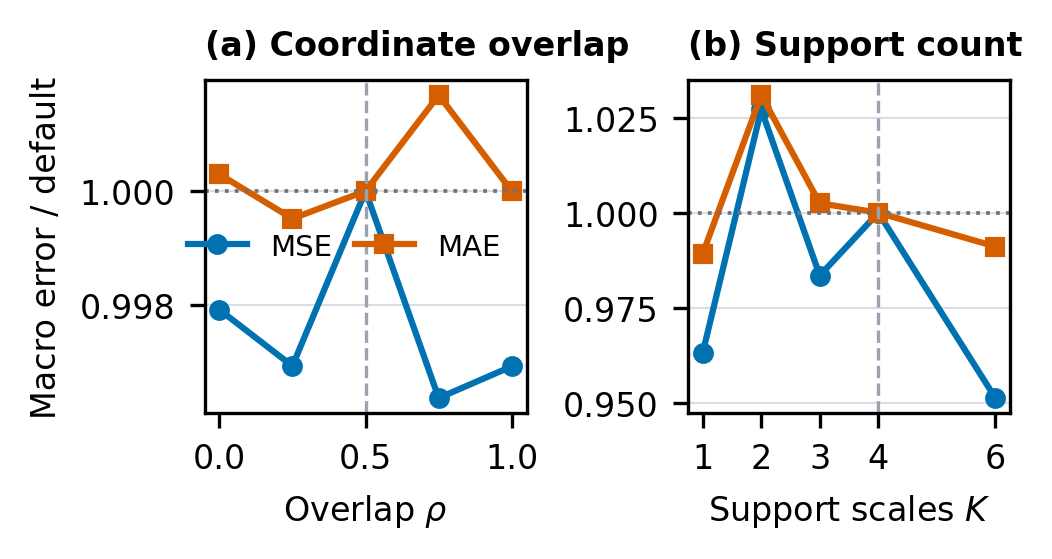
\includegraphics[width=\columnwidth]{figures/final/mesa_fig4_v675_method_sensitivity.png}
\caption{Method-parameter sensitivity on four core datasets. Validation errors
are macro-normalized by the deployed $\rho=0.5$ and $K=4$ setting.}
\label{fig:v675-method}
\end{figure}

Figure~\ref{fig:v675-method} reports one-run validation sensitivity for the
two parameters that directly control
the proposed operator: DCT-subspace overlap $\rho$ and the number of causal
support scales $K$. Varying $\rho$ over $[0,1]$ changes macro MSE/MAE by at
most $0.36\%/0.17\%$. Scale count is more
consequential: relative to $K=4$, macro deviations range from $-4.87\%$ to
$+2.71\%$ MSE and $-1.08\%$ to $+3.09\%$ MAE. No count dominates every
dataset: $K=6$ improves both metrics on HumanActivity and MHEALTH, improves
PAMAP2 MSE while slightly worsening its MAE, and does not help OPPORTUNITY,
whose best validation point is $K=3$. We therefore retain the predeclared
shared $K=4$ rather than adapting $K$ to each test dataset. Exact one-run
validation errors are reported in the supplement.

\subsection{Efficiency}

\begin{table}[t]
\centering
\setlength{\tabcolsep}{2.2pt}
\caption{Efficiency on MHEALTH (batch size 4; lower is better). Par./MACs/Mem. use M/G/GB; Tr./Inf. use ms.}
\label{tab:v665-efficiency}
\begin{tabular}{@{}lrrrrr@{}}
\toprule
Method & Par. & MACs & Mem. & Tr. & Inf. \\
\midrule
APN       & \textbf{.021} & .017 & \textbf{.043} & \textbf{5.81} & \textbf{1.30} \\
KAFNet    & .038 & \textbf{.011} & 4.425 & 10.83 & 3.41 \\
tPatchGNN & .391 & .367 & 3.121 & 81.04 & 32.42 \\
GraFITi   & .498 & 3.670 & 1.192 & 48.35 & 22.77 \\
PatchTST  & .077 & .020 & .050 & 7.27 & 1.81 \\
MESANet   & 1.733 & .305 & .151 & 23.28 & 11.24 \\
\bottomrule
\end{tabular}
\end{table}


Table~\ref{tab:v665-efficiency} compares parameter count, multiply-accumulate
operations (MACs), optimizer-step
peak memory, training latency, and inference latency on one RTX 4080. MESANet
uses 1.733M parameters and 0.305G MACs. Its
23.28-ms training step and 11.24-ms inference step are $2.08\times$ and
$2.03\times$ faster than GraFITi, while its 0.151-GB peak memory is
$7.89\times$ lower. Relative to tPatchGNN it is $3.48\times/2.89\times$
faster and uses $20.65\times$ less peak memory.
PatchTST remains the lowest-cost competitive model. MESANet therefore trades
higher cost than lightweight regular patches for lower cost than the two dense
irregular graph baselines profiled here.

\subsection{Subject and Observation-Mechanism Stress Tests}

\begin{table}[t]
\centering
\setlength{\tabcolsep}{3.0pt}
\caption{Subject-transfer and observation-mask stress results.}
\label{tab:v671-stress}
\begin{tabular}{@{}p{0.34\columnwidth}cc@{}}
\toprule
Protocol & Gain MSE/MAE & Wins MSE/MAE \\
\midrule
LOSO--MH & $+6.76/+7.08\%$ & 10/10; 10/10 \\
LOSO--USC & $+3.96/+4.19\%$ & 13/14; 14/14 \\
Group async. & $+2.98/+3.42\%$ & 3/3; 3/3 \\
Matched MCAR & $+7.78/+10.13\%$ & 3/3; 3/3 \\
Matched block & $+0.27/+2.55\%$ & 2/3; 3/3 \\
\bottomrule
\end{tabular}
\end{table}

Table~\ref{tab:v671-stress} separates two forms of distribution shift from the
main optimization-repeat benchmark. Leave-one-subject-out (LOSO) gains are
geometric means over 10
MHEALTH and 14 USC-HAD subjects; mask gains are arithmetic means over three
datasets. In strict LOSO, every test subject is
excluded from training and validation. Against the predeclared PatchTST
comparator, MESANet improves geometric MSE/MAE by $5.14\%/5.41\%$ over all 24
subjects, with 23/24 and 24/24 wins. The mean log-ratio bootstrap intervals
exclude zero on both MHEALTH and USC-HAD; fold-level errors and intervals are
reported in the supplement. This is evidence of subject transfer, not an
additional optimization-seed claim.

The one-run mask suite replaces released availability with group-asynchronous,
density-matched missing-completely-at-random (MCAR), or density-matched block
masks on MHEALTH, OPPORTUNITY, and PAMAP2. HumanActivity is excluded because
its released loader does not apply these mask-protocol controls. MESANet wins
7/9 MSE and 9/9 MAE cells. The MSE reversals are PAMAP2 under group
asynchrony ($-0.08\%$) and OPPORTUNITY under block removal ($-2.72\%$), while
MAE remains positive. The latter is a boundary under long contiguous gaps in
this run.

Across these experiments, the strongest repeated evidence concerns the frozen
main contrasts and the four-dataset component controls. LOSO measures variation
over held-out subjects with one optimization run per fold, and the mask suite
is a one-run mechanism stress test. They define transfer and missingness
boundaries rather than extend the five-run paired optimization-run comparison.
